Implicitly underlying benchmarking for solvers is the following hypothesis.
\begin{hypothesis}Our solvers will be faced in practice (read ``the next competition'') with problems whose time-to-solve distribution is the same as that for the benchmark set.
\end{hypothesis}
A necessary condition is that one has a large benchmark set, ideally in the thousands. Sampling appropriately is always a question of judgement.
\begin{figure}[h]
\caption{A Survival Plot\label{fig:survivor}}
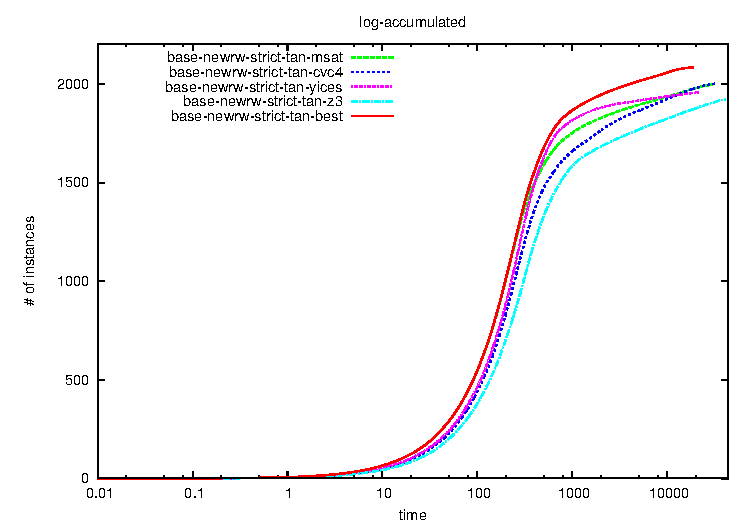
\includegraphics{log-accumulated2.pdf}
\vskip-0pt
\end{figure}
\section{``Cactus'' or ``Survival'' plots}
Figure \ref{fig:survivor} is a typical survival\footnote{``Cactus'' plots are the same with the axes flipped. Some cactus plots can be seen at \url{http://fmv.jku.at/hwmcc15/Biere-HWMCC15-talk.pdf}, exept that these aren't cumulative, i.e. $(k,t_k)$ was plotted.} plot produced in the SMT community.
The methodology for producing these, given a large benchmark set of problems, is as follows.
\begin{enumerate}
\item For each method separately
\begin{enumerate}
\item Solve each problem $p_i$, noting the time $t_i$ (up to some threshold $T$).
\item Sort the $t_i$ into increasing order (discarding the time-out ones).
\item Plot the points $(t_1,1)$, $(t_1+t_2,2)$ etc., and in general $(\sum_{i=1}^kt_i,k)$.
\end{enumerate}
\item Place all the plots on the same axes, optionally (as in Figure \ref{fig:survivor}) using a logarithmic scale for time.
\item[N.B.]There is therefore no guarantee that the same problems were used to produce time results from different solvers.
\end{enumerate}
From \ref{fig:survivor} we can deduce that, up to 100 seconds, the solvers are pretty similar, and with a time budget of 100 seconds, can solve \emph{at most} around 500 problems. At a time budget of 1000 seconds, the differences are more marked, and the worst solved around 1600 problems and the best around 2000.
\section{CDF plots}
An alternative is (still after sorting the $t_i$) to plot  $(t_1,1)$, $(t_2,2)$ etc., and in general $(t_k,k)$. If we normalise the $y$ axis to $[0,1]$ (\emph{not} discarding the timeouts) we have an approximation to the cumulative distribution function. See \cite{Xuetal2008b} for some examples. Hence from these plots we can ask questions like ``what is the probability of solving a random problem in $t$ seconds''.
